\begin{answer}
The region for class 1(marked as x) is the union of three halfspaces, $x_1<0.5$, $x_2<0.5$, and $x_1+x_2>4$. Therefore the network can achieve 100\% accuracy if we let each node classify whether the node is in one halfspace(one node for each halfspace). Then, the output layer returns 1 if the input is in at least one of the halfspaces.
\begin{figure}[H]
    \centering
    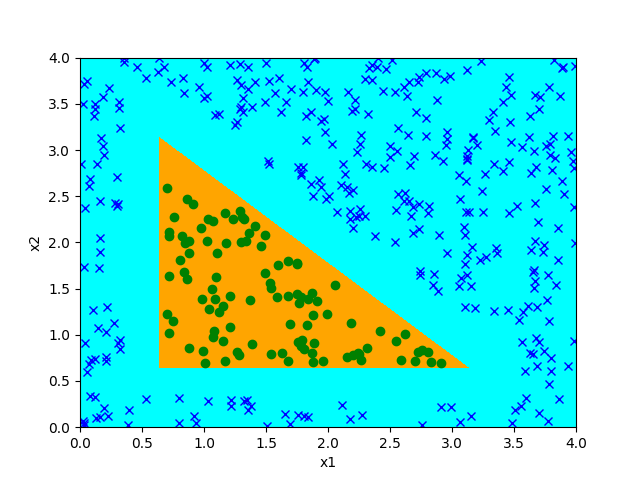
\includegraphics[width=9cm]{simple_nn/step_weights.png}
\end{figure}
\end{answer}
